\section{State-Space Search Problems}
\label{sec:state-space-search}

In state-space search problems, the environment is represented through \textbf{states} that must be uniquely distinguishable from each other, but lack accessible characteristics that allow direct differentiation. For the agent, they are simply different "labels" representing distinct states.

\subsection{Problem Components}
\label{subsec:problem-components}

This type of problem is defined by three essential elements:

\begin{itemize}
    \item \textbf{State space}: A model of the world represented by a graph, where nodes represent components of the world. These components are translated into elements of the symbolic model, symbolized in a specific way within the graph.
    
    \item \textbf{Search problem}: Through a problem-independent mechanism, we explore the state space by applying the agent's attitude, which represents the rationality component in the exploration process.
    
    \item \textbf{Objective}: To find the most efficient plan that leads from the initial state to a goal state.
\end{itemize}

\subsection{The Search Challenge}
\label{subsec:search-challenge}

Therefore, this type of problem aims to find the best path within a directed graph, as shown in Figure~\ref{fig:state-space-graph}. However, we do not know the graph structure in advance. If we knew it, we could perform a minimum path search using algorithms like Dijkstra's algorithm.

\begin{figure}[H]
    \centering
    \includegraphics[width=0.9\textwidth]{img/graph.png}
    \caption{Example of a state-space search graph. The red nodes and path highlight a possible solution path from the initial state (s1) to a goal state (s12).}
    \label{fig:state-space-graph}
\end{figure}

Since the graph is unknown, we must explore it incrementally through search algorithms, discovering states and transitions as we explore the state space.

\subsection{The Search Process}
\label{subsec:search-process}

The search method operates through an iterative cycle, as illustrated in Figure~\ref{fig:search-method}:

\begin{figure}[H]
    \centering
    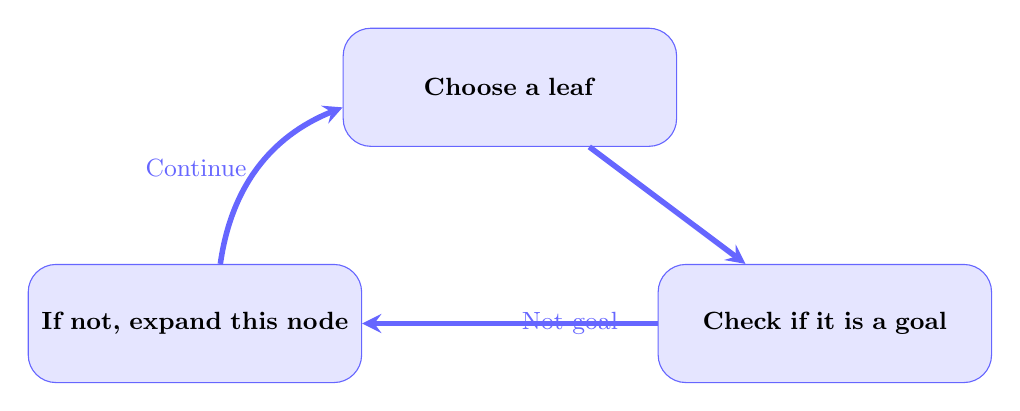
\begin{tikzpicture}[
        box/.style={rectangle, rounded corners=10pt, draw=blue!60, fill=blue!10, text width=4cm, minimum height=1.5cm, align=center, font=\small},
        arrow/.style={->, >=stealth, blue!60, line width=2pt}
    ]
        % Boxes
        \node[box] (choose) at (0,0) {\textbf{Choose a leaf}};
        \node[box] (check) at (4,-3) {\textbf{Check if it is a goal}};
        \node[box] (expand) at (-4,-3) {\textbf{If not, expand this node}};
        
        % Arrows
        \draw[arrow] (choose) -- (check);
        \draw[arrow] (check) -- node[right, font=\small] {Not goal} (expand);
        \draw[arrow, bend left=30] (expand) to node[left, font=\small] {Continue} (choose);
    \end{tikzpicture}
    \caption{Search method based on the selection of a leaf representing a state.}
    \label{fig:search-method}
\end{figure}

The process repeats until a goal state is found. During this exploration, we build a \textbf{search tree} that represents the states we have discovered and explored, as shown in Figure~\ref{fig:search-tree}.

\begin{figure}[H]
    \centering
    \includegraphics[width=0.9\textwidth]{img/tree.png}
    \caption{Example of a search tree showing the exploration of states. Each node represents a state configuration, and edges represent transitions between states.}
    \label{fig:search-tree}
\end{figure}

\begin{figure}[H]
    \centering
    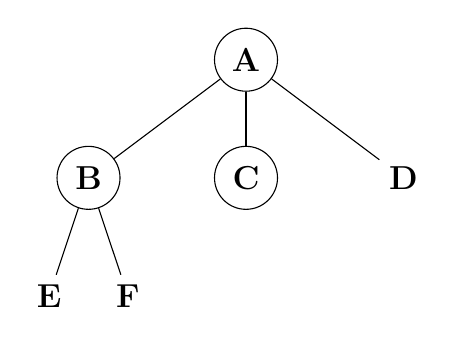
\begin{tikzpicture}[
        node/.style={circle, draw=black, fill=white, minimum size=0.8cm, font=\large\bfseries},
        textnode/.style={font=\large\bfseries}
    ]
        % Tree nodes
        \node[node] (A) at (0,0) {A};
        \node[node] (B) at (-2,-1.5) {B};
        \node[node] (C) at (0,-1.5) {C};
        \node[textnode] (D) at (2,-1.5) {D};
        \node[textnode] (E) at (-2.5,-3) {E};
        \node[textnode] (F) at (-1.5,-3) {F};
        
        % Edges
        \draw (A) -- (B);
        \draw (A) -- (C);
        \draw (A) -- (D);
        \draw (B) -- (E);
        \draw (B) -- (F);
    \end{tikzpicture}
    \caption{Nomenclature for graph traversal in search algorithms. \textbf{Notation:} When expanding, we note the successors from left to right, but the algorithm does not always expand them in that order (another algorithm could have chosen D before, and would then continue on that side of the figure).}
    \label{fig:search-nomenclature}
\end{figure}

\textit{It is a particular way of traversing a graph (it will be different for each algorithm we will see).}

\begin{itemize}
    \item \textbf{A} is a node with initial state (expanded) with three successors B, C, D.
    \item \textbf{B} is a node with state B, expanded, with two successors.
    \item \textbf{C} is a node with state C, expanded, without successors.
    \item \textbf{D} is a node pending expansion (in open list).
    \item \textbf{E} is a node pending expansion (in open list).
    \item \textbf{F} is a node pending expansion (in open list).
\end{itemize}

\subsection{General Search Algorithm}
\label{subsec:general-search-algorithm}

We can define a general search algorithm as shown in the following Python implementation:

\begin{lstlisting}[caption={General search algorithm}, label={lst:general-search}]
def general_search(initial_state, goal_state):
    """
    General search algorithm for state-space problems.
    
    Args:
        initial_state: The starting state S0
        goal_state: The goal state G
    
    Returns:
        Path from initial_state to goal_state, or None if no solution exists
    """
    # Line 1: Initialize open list with initial state
    open_list = [Node(initial_state, parent=None)]
    
    # Line 2: Main search loop
    while open_list:  # While open_list is not empty
        # Line 3: Extract first node from open list
        node = open_list.pop(0)  # FIFO for BFS
        
        # Line 4-5: Check if node is goal
        if is_goal(node.state, goal_state):
            # Return path by backtracking through parent nodes
            return reconstruct_path(node)
        
        # Line 7: Expand node to get successors
        successors = expand(node.state)
        
        # Line 8-10: Add successors to open list
        for successor_state in successors:
            successor_node = Node(successor_state, parent=node)
            open_list.append(successor_node)
    
    # Line 13: No solution found
    return None

class Node:
    """Node representation in the search tree."""
    def __init__(self, state, parent=None):
        self.state = state  # State reached at this point
        self.parent = parent  # Reference to parent node (line 9)
\end{lstlisting}

\subsubsection{Algorithm Components}
\label{subsubsec:algorithm-components}

The search tree is represented using a \textbf{Node} record type. In its simplest form, a node is linked to its predecessor (parent) through a reference (line 112 in the code, where the parent is set in the Node constructor). Each node stores the state reached at that point in the exploration.

\begin{itemize}
    \item \textbf{Open list} (line 85): A list of nodes containing the current leaves of the tree—those states and paths that have been expanded for exploration.
    
    \item \textbf{Empty list check} (line 88): If the list is empty, we have encountered a problem with no solution. Otherwise, we extract the first element from the list of open leaves (line 90).
    
    \item \textbf{Goal check} (lines 93-95): If the node is a goal state, we return the path by performing backtracking through the parent nodes of the found goal node.
    
    \item \textbf{Expansion} (lines 98, 101-103): We expand the node to get successors (line 98), then add the new states obtained from expansion to the open list (lines 101-103).
\end{itemize}

In the following sections, we will show how different uninformed search algorithms work, which are used as the foundation for many intelligent agent problems.

\subsubsection{Repeated States Problem}
\label{subsubsec:repeated-states}

In all search mechanisms, we face a potential problem: \textbf{repeated states}. This can cause serious errors in some cases, such as entering infinite loops. We have different strategies to resolve this:

\begin{itemize}
    \item \textbf{Ignore it}: As strange as it may seem, some algorithms do not have problems with this solution due to their own exploration order.
    
    \item \textbf{Avoid simple cycles}: Prevent adding the parent of a node to the set of successors.
    
    \item \textbf{Avoid general cycles}: Prevent any ancestor of a node from being added to the set of successors.
    
    \item \textbf{Avoid all repeated states}: Do not allow adding any node that already exists in the tree to the set of successors.
\end{itemize}

These strategies must consider the cost of both exploring too much and searching for repeated elements to explore less. The choice depends on the specific problem and the trade-off between memory usage and computational efficiency.

\subsection{Algorithm Classification Criteria}
\label{subsec:algorithm-classification}

In the following sections, we will present different search algorithms. For all of them, we will use a classification mechanism based on the following concepts and characteristics:

\subsubsection{Completeness}
\label{subsubsec:completeness}

An algorithm is \textbf{complete} if it is guaranteed to find a solution whenever one exists. If no solution exists, a complete algorithm will correctly report that no solution was found.

\textit{Example}: Imagine you're searching for your keys in your house. A complete search method would guarantee that if your keys are somewhere in the house, you will eventually find them. If you search room by room systematically, you're using a complete method. However, if you only check the living room and give up, that's an incomplete method—you might miss the keys if they're in the bedroom.

\subsubsection{Optimality}
\label{subsubsec:optimality}

An algorithm is \textbf{optimal} if, when multiple solutions exist, it always finds the best one according to some cost measure (e.g., shortest path, minimum number of steps, lowest cost).

\textit{Example}: Consider finding a route from your home to a restaurant. There might be three routes: Route A (5 km, 10 minutes), Route B (8 km, 8 minutes), and Route C (12 km, 15 minutes). An optimal algorithm would find Route B if you want the fastest route, or Route A if you want the shortest distance. A non-optimal algorithm might find Route C first and stop there, even though better options exist.

\subsubsection{Time Complexity}
\label{subsubsec:time-complexity}

\textbf{Time complexity} measures how long an algorithm takes to find a solution, typically expressed in terms of the problem size (e.g., number of nodes, depth of the search tree).

\textit{Example}: Think of searching for a specific book in a library. If the library has 1,000 books and you check them one by one, you might need to check all 1,000 in the worst case. If the library has 10,000 books, you might need to check all 10,000. The time complexity describes how the search time grows as the library size increases. Some algorithms might need to explore exponentially more states as the problem grows, while others scale more efficiently.

\subsubsection{Space Complexity}
\label{subsubsec:space-complexity}

\textbf{Space complexity} measures how much memory an algorithm requires to find a solution. This includes the storage needed for the open list, closed list, and other data structures.

\textit{Example}: Imagine you're exploring a maze and want to remember all the paths you've tried. A method that stores every path you've explored requires more memory than one that only remembers the current path. If the maze is very large, storing all explored paths might require more memory than your computer has available. Space complexity helps us understand these memory requirements and choose algorithms that fit within available resources.
